
\documentclass[letterpaper,hide notes,xcolor={table,svgnames},pdftex,10pt]{beamer}
\def\showexamples{t}


%\usepackage[svgnames]{xcolor}

%% Demo talk
%\documentclass[letterpaper,notes=show]{beamer}

\usecolortheme{crane}
\setbeamertemplate{navigation symbols}{}

\usetheme{MyPittsburgh}
%\usetheme{Frankfurt}

%\usepackage{tipa}

\usepackage{hyperref}
\usepackage{graphicx,xspace}
\usepackage[normalem]{ulem}
\usepackage{multicol}
\usepackage{amsmath,amssymb,amsthm,graphicx,xspace}
\newcommand\SF[1]{$\bigstar$\footnote{SF: #1}}

\usepackage[default]{sourcesanspro}
\usepackage[T1]{fontenc}
\usepackage[scaled]{beramono}
\usepackage{tikzpagenodes}

\newcounter{tmpnumSlide}
\newcounter{tmpnumNote}


% old question code
%\newcommand\question[1]{{$\bigstar$ \small \onlySlide{2}{#1}}}
% \newcommand\nquestion[1]{\ifdefined \presentationonly \textcircled{?} \fi \note{\par{\Large \textbf{?}} #1}}
% \newcommand\nanswer[1]{\note{\par{\Large \textbf{A}} #1}}


 \newcommand\mnote[1]{%
   \addtocounter{tmpnumSlide}{1}
   \ifdefined\showcues {~\tiny\fbox{\arabic{tmpnumSlide}}}\fi
   \note{\setlength{\parskip}{1ex}\addtocounter{tmpnumNote}{1}\textbf{\Large \arabic{tmpnumNote}:} {#1\par}}}

\newcommand\mmnote[1]{\note{\setlength{\parskip}{1ex}#1\par}}

%\newcommand\mnote[2][]{\ifdefined\handoutwithnotes {~\tiny\fbox{#1}}\fi
% \note{\setlength{\parskip}{1ex}\textbf{\Large #1:} #2\par}}

%\newcommand\mnote[2][]{{\tiny\fbox{#1}} \note{\setlength{\parskip}{1ex}\textbf{\Large #1:} #2\par}}

\newcommand\mquestion[2]{{~\color{red}\fbox{?}}\note{\setlength{\parskip}{1ex}\par{\Large \textbf{?}} #1} \note{\setlength{\parskip}{1ex}\par{\Large \textbf{A}} #2\par}\ifdefined \presentationonly \pause \fi}

\newcommand\blackboard[1]{%
\ifdefined   \showblackboard
  {#1}
  \else {\begin{center} \fbox{\colorbox{blue!30}{%
         \begin{minipage}{.95\linewidth}%
           \hspace{\stretch{1}} Some space intentionally left blank; done at the blackboard.%
         \end{minipage}}}\end{center}}%
         \fi%
}



%\newcommand\q{\tikz \node[thick,color=black,shape=circle]{?};}
%\newcommand\q{\ifdefined \presentationonly \textcircled{?} \fi}

\usepackage{listings}
\lstset{basicstyle=\footnotesize\ttfamily,
	breaklines=true,
	aboveskip=15pt,
  	belowskip=15pt,
	frame=lines,
	numbers=left, basicstyle=\scriptsize, numberstyle=\tiny, stepnumber=0, numbersep=2pt
}

\usepackage{siunitx}
\newcommand\sius[1]{\num[group-separator = {,}]{#1}\si{\micro\second}}
\newcommand\sims[1]{\num[group-separator = {,}]{#1}\si{\milli\second}}
\newcommand\sins[1]{\num[group-separator = {,}]{#1}\si{\nano\second}}
\sisetup{group-separator = {,}, group-digits = true}

%% -------------------- tikz --------------------
\usepackage{tikz}
\usetikzlibrary{positioning}
\usetikzlibrary{arrows,backgrounds,automata,decorations.shapes,decorations.pathmorphing,decorations.markings,decorations.text,decorations.pathreplacing}

\tikzstyle{place}=[circle,draw=blue!50,fill=blue!20,thick, inner sep=0pt,minimum size=6mm]
\tikzstyle{transition}=[rectangle,draw=black!50,fill=black!20,thick, inner sep=0pt,minimum size=4mm]

\tikzstyle{block}=[rectangle,draw=black, thick, inner sep=5pt]
\tikzstyle{bullet}=[circle,draw=black, fill=black, thin, inner sep=2pt]

\tikzstyle{pre}=[<-,shorten <=1pt,>=stealth',semithick]
\tikzstyle{post}=[->,shorten >=1pt,>=stealth',semithick]
\tikzstyle{bi}=[<->,shorten >=1pt,shorten <=1pt, >=stealth',semithick]

\tikzstyle{mut}=[-,>=stealth',semithick]

\tikzstyle{treereset}=[dashed,->, shorten >=1pt,>=stealth',thin]

\usepackage{ifmtarg}
\usepackage{xifthen}
\makeatletter
% new counter to now which frame it is within the sequence
\newcounter{multiframecounter}
% initialize buffer for previously used frame title
\gdef\lastframetitle{\textit{undefined}}
% new environment for a multi-frame
\newenvironment{multiframe}[1][]{%
\ifthenelse{\isempty{#1}}{%
% if no frame title was set via optional parameter,
% only increase sequence counter by 1
\addtocounter{multiframecounter}{1}%
}{%
% new frame title has been provided, thus
% reset sequence counter to 1 and buffer frame title for later use
\setcounter{multiframecounter}{1}%
\gdef\lastframetitle{#1}%
}%
% start conventional frame environment and
% automatically set frame title followed by sequence counter
\begin{frame}%
\frametitle{\lastframetitle~{\normalfont(\arabic{multiframecounter})}}%
}{%
\end{frame}%
}
\makeatother

\makeatletter
\newdimen\tu@tmpa%
\newdimen\ydiffl%
\newdimen\xdiffl%
\newcommand\ydiff[2]{%
    \coordinate (tmpnamea) at (#1);%
    \coordinate (tmpnameb) at (#2);%
    \pgfextracty{\tu@tmpa}{\pgfpointanchor{tmpnamea}{center}}%
    \pgfextracty{\ydiffl}{\pgfpointanchor{tmpnameb}{center}}%
    \advance\ydiffl by -\tu@tmpa%
}
\newcommand\xdiff[2]{%
    \coordinate (tmpnamea) at (#1);%
    \coordinate (tmpnameb) at (#2);%
    \pgfextractx{\tu@tmpa}{\pgfpointanchor{tmpnamea}{center}}%
    \pgfextractx{\xdiffl}{\pgfpointanchor{tmpnameb}{center}}%
    \advance\xdiffl by -\tu@tmpa%
}
\makeatother
\newcommand{\copyrightbox}[3][r]{%
\begin{tikzpicture}%
\node[inner sep=0pt,minimum size=2em](ciimage){#2};
\usefont{OT1}{phv}{n}{n}\fontsize{4}{4}\selectfont
\ydiff{ciimage.south}{ciimage.north}
\xdiff{ciimage.west}{ciimage.east}
\ifthenelse{\equal{#1}{r}}{%
\node[inner sep=0pt,right=1ex of ciimage.south east,anchor=north west,rotate=90]%
{\raggedleft\color{black!50}\parbox{\the\ydiffl}{\raggedright{}#3}};%
}{%
\ifthenelse{\equal{#1}{l}}{%
\node[inner sep=0pt,right=1ex of ciimage.south west,anchor=south west,rotate=90]%
{\raggedleft\color{black!50}\parbox{\the\ydiffl}{\raggedright{}#3}};%
}{%
\node[inner sep=0pt,below=1ex of ciimage.south west,anchor=north west]%
{\raggedleft\color{black!50}\parbox{\the\xdiffl}{\raggedright{}#3}};%
}
}
\end{tikzpicture}
}


%% --------------------

%\usepackage[excludeor]{everyhook}
%\PushPreHook{par}{\setbox0=\lastbox\llap{MUH}}\box0}

%\vspace*{\stretch{1}

%\setbox0=\lastbox \llap{\textbullet\enskip}\box0}

\setlength{\parskip}{\fill}

\newcommand\noskips{\setlength{\parskip}{1ex}}
\newcommand\doskips{\setlength{\parskip}{\fill}}

\newcommand\xx{\par\vspace*{\stretch{1}}\par}
\newcommand\xxs{\par\vspace*{2ex}\par}
\newcommand\tuple[1]{\langle #1 \rangle}
\newcommand\code[1]{{\sf \footnotesize #1}}
\newcommand\ex[1]{\uline{Example:} \ifdefined \presentationonly \pause \fi
  \ifdefined\showexamples#1\xspace\else{\uline{\hspace*{2cm}}}\fi}

\newcommand\ceil[1]{\lceil #1 \rceil}


\AtBeginSection[]
{
   \begin{frame}
       \frametitle{Outline}
       \tableofcontents[currentsection]
   \end{frame}
}



\pgfdeclarelayer{edgelayer}
\pgfdeclarelayer{nodelayer}
\pgfsetlayers{edgelayer,nodelayer,main}

\tikzstyle{none}=[inner sep=0pt]
\tikzstyle{rn}=[circle,fill=Red,draw=Black,line width=0.8 pt]
\tikzstyle{gn}=[circle,fill=Lime,draw=Black,line width=0.8 pt]
\tikzstyle{yn}=[circle,fill=Yellow,draw=Black,line width=0.8 pt]
\tikzstyle{empty}=[circle,fill=White,draw=Black]
\tikzstyle{bw} = [rectangle, draw, fill=blue!20, 
    text width=4em, text centered, rounded corners, minimum height=2em]
    
    \newcommand{\CcNote}[1]{% longname
	This work is licensed under the \textit{Creative Commons #1 3.0 License}.%
}
\newcommand{\CcImageBy}[1]{%
	\includegraphics[scale=#1]{creative_commons/cc_by_30.pdf}%
}
\newcommand{\CcImageSa}[1]{%
	\includegraphics[scale=#1]{creative_commons/cc_sa_30.pdf}%
}
\newcommand{\CcImageNc}[1]{%
	\includegraphics[scale=#1]{creative_commons/cc_nc_30.pdf}%
}
\newcommand{\CcGroupBySa}[2]{% zoom, gap
	\CcImageBy{#1}\hspace*{#2}\CcImageNc{#1}\hspace*{#2}\CcImageSa{#1}%
}
\newcommand{\CcLongnameByNcSa}{Attribution-NonCommercial-ShareAlike}

\newenvironment{changemargin}[1]{% 
  \begin{list}{}{% 
    \setlength{\topsep}{0pt}% 
    \setlength{\leftmargin}{#1}% 
    \setlength{\rightmargin}{1em}
    \setlength{\listparindent}{\parindent}% 
    \setlength{\itemindent}{\parindent}% 
    \setlength{\parsep}{\parskip}% 
  }% 
  \item[]}{\end{list}} 




\title{Lecture 30 --- Clusters \& Cloud Computing}

\author{Patrick Lam \\ \small \texttt{patrick.lam@uwaterloo.ca}}
\institute{Department of Electrical and Computer Engineering \\
  University of Waterloo}
\date{\today}


\begin{document}

\begin{frame}
  \titlepage

 \end{frame}


%%%%%%%%%%%%%%%%%%%%%%%%%%%%%%%%%%%%%%%%%%%%%%%%%%%%%%%%%%%%%%%%%%%%%%%%%%%%%%%%
\begin{frame}
  \frametitle{More, More, More}

  

  So far, we've seen how to make things fast on one computer:
\begin{itemize}
\item threads;
\item compiler optimizations;
\item GPUs.
\end{itemize}
  To get a lot of bandwidth, though, you need lots of computers, \\
   \qquad (if you're lucky and the problem allows!)\\[1em]
   
\end{frame}


\begin{frame}
  \frametitle{More, More, More}
  
  \begin{center}
	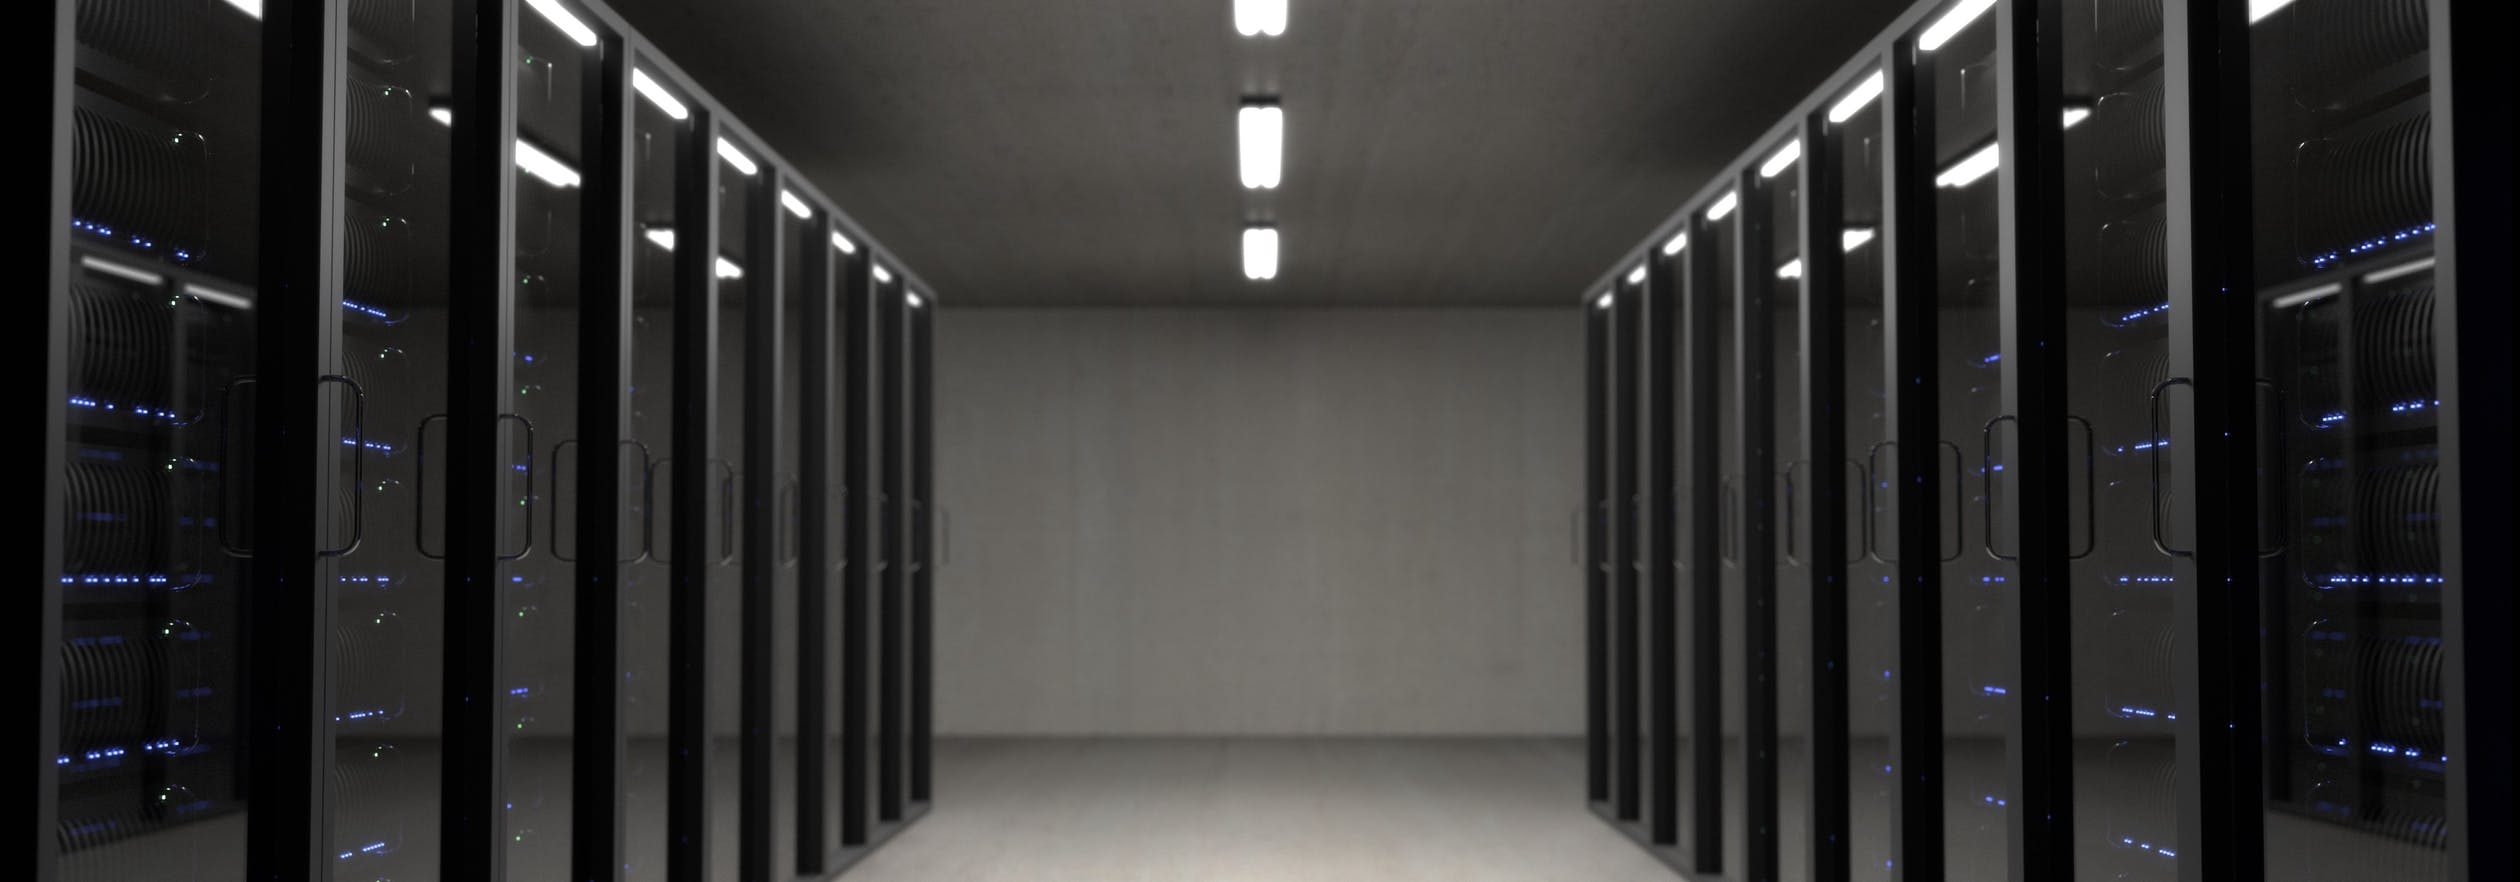
\includegraphics[width= \textwidth]{images/servers.jpeg}
\end{center}

  Today: programming for performance with multiple computers.

  
\end{frame}
%%%%%%%%%%%%%%%%%%%%%%%%%%%%%%%%%%%%%%%%%%%%%%%%%%%%%%%%%%%%%%%%%%%%%%%%%%%%%%%%

%%%%%%%%%%%%%%%%%%%%%%%%%%%%%%%%%%%%%%%%%%%%%%%%%%%%%%%%%%%%%%%%%%%%%%%%%%%%%%%%
\begin{frame}
  \frametitle{Key Idea: Explicit Communication}

  Rust encourages message-passing, but a lot of your previous experience when working with C may have centred around shared memory systems.
  
	Sometimes: no choice! Such as GPU.

  Recently, GPU programming: explicitly copy data.

Communication over the network is much more expensive than within the same system.

  
\end{frame}
%%%%%%%%%%%%%%%%%%%%%%%%%%%%%%%%%%%%%%%%%%%%%%%%%%%%%%%%%%%%%%%%%%%%%%%%%%%%%%%%

%%%%%%%%%%%%%%%%%%%%%%%%%%%%%%%%%%%%%%%%%%%%%%%%%%%%%%%%%%%%%%%%%%%%%%%%%%%%%%%%
\begin{frame}
  \frametitle{What is MPI?}

\begin{center}
	
\includegraphics[width=0.3\textwidth]{images/mpi.png}
\end{center}
  {\bf Message Passing Interface:}

  A language-independent communation protocol\\ for parallel computers.

This is, unfortunately, no longer the way. 
  
\end{frame}
%%%%%%%%%%%%%%%%%%%%%%%%%%%%%%%%%%%%%%%%%%%%%%%%%%%%%%%%%%%%%%%%%%%%%%%%%%%%%%%%




\begin{frame}
\frametitle{REST}

We've already seen asynchronous I/O using HTTP (curl) $\rightarrow$ REST!

You may have also learned about sockets $\rightarrow$ too low level.

The REST API approach is at a reasonable level of abstraction. 

\end{frame}


\begin{frame}
\frametitle{Synchronous REST}

REST APIs are often completely synchronous, but don't have to be:

You can set up  callbacks or check back later.

The remote machine has to be available at the time of each call...

\end{frame}


\begin{frame}
\frametitle{Kafka}

\begin{center}
	
\includegraphics[width=0.4\textwidth]{images/kafkalogo.png}
\end{center}


Apache Kafka: a self-described ``distributed streaming platform''.

\end{frame}


\begin{frame}
\frametitle{Kafka}

Producers write a record into a topic and consumers take the item from the topic and doing something useful with it.

A message remains available for a fixed period of time and can be replayed if needed.

Publish-subscribe model.

\end{frame}



\begin{frame}
\frametitle{Change is Hard}

Kafka's basic strategy is to write things into an immutable log. 

The log is split into different partitions.

Consumers read from each one of the partitions and writes down its progress.

\begin{center}
	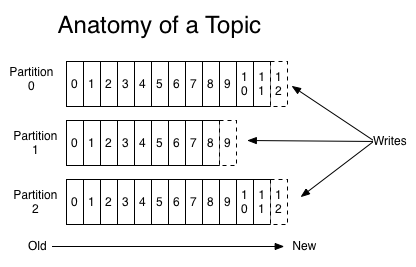
\includegraphics[width=0.7\textwidth]{images/kafka-partition.png}
\end{center}


\end{frame}


\begin{frame}
\frametitle{Kafka Provisioning}

We can provision the parallelism that we want, and the logic for the broker.

Consumers can take items and deal with them at their own speed.

Messages are removed from the topic based on their expiry.

\end{frame}


\begin{frame}
\frametitle{Hurry up and Queue}

In something like a standard queue, there's a little bit of pressure to get items out of the queue quickly.

You might think that it's a solution to take the item out of the queue in one transaction and then process it later.

That's okay only if you've successfully saved it to a database or other persistent storage. 

\end{frame}


\begin{frame}
\frametitle{Alternatives: SQS and SNS}

SNS (Simple Notification Service) and SQS (Simple Queueing Service). 

They are, broadly speaking, just other ways to decouple the communication of your programs.

SNS is good for sending lots of messages to multiple receivers.

SQS is more for batches of work where it's not particularly time-sensitive and the item will be consumed by a worker.

\end{frame}


\begin{frame}
\frametitle{How would you know the difference?}
\begin{center}
	
\includegraphics[width=0.6\textwidth]{images/thecloud.jpg}
\end{center}
\end{frame}

%%%%%%%%%%%%%%%%%%%%%%%%%%%%%%%%%%%%%%%%%%%%%%%%%%%%%%%%%%%%%%%%%%%%%%%%%%%%%%%%
\begin{frame}
  \frametitle{Using a Cluster}

  
    Historically:
\begin{itemize}
  \item find \$\$\$;
  \item buy and maintain pile of expensive machines.
\end{itemize}

  Not anymore! \\[1em]

  We'll talk about Amazon's Elastic Compute Cloud (EC2)\\ and
  principles behind it.
  
\end{frame}
%%%%%%%%%%%%%%%%%%%%%%%%%%%%%%%%%%%%%%%%%%%%%%%%%%%%%%%%%%%%%%%%%%%%%%%%%%%%%%%%

%%%%%%%%%%%%%%%%%%%%%%%%%%%%%%%%%%%%%%%%%%%%%%%%%%%%%%%%%%%%%%%%%%%%%%%%%%%%%%%%
\begin{frame}
  \frametitle{Evolution of servers}

  

You want a server on the Internet.
\begin{itemize}
\item 
  Once upon a time: physical machine; shared hosting.
\item Virtualization:
\item Clouds
\end{itemize}

  Servers typically share persistent storage, also in
  the cloud. 

  
\end{frame}
%%%%%%%%%%%%%%%%%%%%%%%%%%%%%%%%%%%%%%%%%%%%%%%%%%%%%%%%%%%%%%%%%%%%%%%%%%%%%%%%

%%%%%%%%%%%%%%%%%%%%%%%%%%%%%%%%%%%%%%%%%%%%%%%%%%%%%%%%%%%%%%%%%%%%%%%%%%%%%%%%
\begin{frame}
  \frametitle{Paying for Computes}

  
Cloud computing: pay by the number of
instances that you've started up.


Providers offer different instance sizes: vary in cores, memory, GPU...

  
\end{frame}
%%%%%%%%%%%%%%%%%%%%%%%%%%%%%%%%%%%%%%%%%%%%%%%%%%%%%%%%%%%%%%%%%%%%%%%%%%%%%%%%

%%%%%%%%%%%%%%%%%%%%%%%%%%%%%%%%%%%%%%%%%%%%%%%%%%%%%%%%%%%%%%%%%%%%%%%%%%%%%%%%
\begin{frame}
  \frametitle{Launching Instances}
  
  \begin{center}
	
\includegraphics[width=0.4\textwidth]{images/kirk.png}
\end{center}

  
Need more computes? Launch an instance!\\[1em]

Input: Virtual Machine image.\\[1em]

Mechanics: use a command-line or web-based tool.\\[1em]

New instance gets an IP address and is network-accessible. \\
You have full root access to that instance.
  
\end{frame}
%%%%%%%%%%%%%%%%%%%%%%%%%%%%%%%%%%%%%%%%%%%%%%%%%%%%%%%%%%%%%%%%%%%%%%%%%%%%%%%%

%%%%%%%%%%%%%%%%%%%%%%%%%%%%%%%%%%%%%%%%%%%%%%%%%%%%%%%%%%%%%%%%%%%%%%%%%%%%%%%%
\begin{frame}
  \frametitle{What to Launch?}

  
Amazon provides public images:
\begin{itemize}
\item different Linux distributions;
\item Windows Server; and
\item OpenSolaris (maybe not anymore?). 
\end{itemize}

You can build an image which contains software you
want, including Hadoop and OpenMPI.
  
\end{frame}
%%%%%%%%%%%%%%%%%%%%%%%%%%%%%%%%%%%%%%%%%%%%%%%%%%%%%%%%%%%%%%%%%%%%%%%%%%%%%%%%

%%%%%%%%%%%%%%%%%%%%%%%%%%%%%%%%%%%%%%%%%%%%%%%%%%%%%%%%%%%%%%%%%%%%%%%%%%%%%%%%
\begin{frame}
  \frametitle{Cleanup}

  
Presumably you don't want to pay forever for your instances.\\[1em]

When you're done with an instance:

\begin{center}
	
\includegraphics[width=0.3\textwidth]{images/shutitdown.jpg}
\end{center}


All data on instance goes away.
  
\end{frame}

%%%%%%%%%%%%%%%%%%%%%%%%%%%%%%%%%%%%%%%%%%%%%%%%%%%%%%%%%%%%%%%%%%%%%%%%%%%%%%%%

%%%%%%%%%%%%%%%%%%%%%%%%%%%%%%%%%%%%%%%%%%%%%%%%%%%%%%%%%%%%%%%%%%%%%%%%%%%%%%%%
\begin{frame}
  \frametitle{Data Storage}
  
To keep persistent results:
\begin{itemize}
\item mount a storage device,
also on the cloud (e.g. Amazon Elastic Block Storage); or, 
\item connect to a database on a persistent server (e.g. Amazon SimpleDB or
Relational Database Service); or, 
\item you can store files on the Web (e.g. Amazon S3). 
\end{itemize}
  
\end{frame}
%%%%%%%%%%%%%%%%%%%%%%%%%%%%%%%%%%%%%%%%%%%%%%%%%%%%%%%%%%%%%%%%%%%%%%%%%%%%%%%%


\begin{frame}
\frametitle{Clusters vs. Laptops}


\begin{changemargin}{1cm}
Key idea: scaling to big data systems \\
introduces substantial overhead. \\[1em]
Up next: Laptop vs. 128-core big data systems.
\end{changemargin}

\end{frame}



\begin{frame}
\frametitle{Don't Guess, Measure}


\begin{changemargin}{1cm}
Are big data systems obviously good?\\
Have we measured (the right thing)?\\[1em]

The important metric is not just scalability; \\
absolute performance matters a lot. 

\end{changemargin}

\end{frame}



\begin{frame}
\frametitle{Why Scale?}


\begin{changemargin}{1cm}
Don't want: scaling up to $n$ systems \\
to deal with complexity of scaling up to $n$.\\[1em]

\begin{center}
	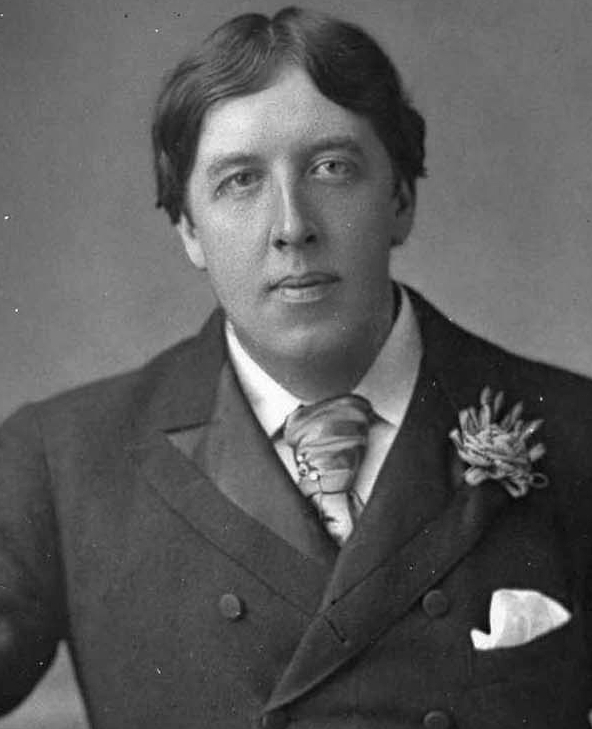
\includegraphics[width=0.3\textwidth]{images/wilde.jpg}
\end{center}

Or, as Oscar Wilde put it: \\
``The bureaucracy is expanding to meet the needs of the expanding bureaucracy.''
\end{changemargin}
\end{frame}



\begin{frame}
\frametitle{Methodology}


\begin{changemargin}{1cm}
Compare: competent single-threaded implementation vs. top
big data systems. 

Domain: graph processing
algorithms---
PageRank and graph connectivity \\
(bottleneck is label propagation). 

Subjects: graphs with billions of edges\\
(a few
GB of data.)
\end{changemargin}

\end{frame}



\begin{frame}
\frametitle{Results}

\begin{center}
	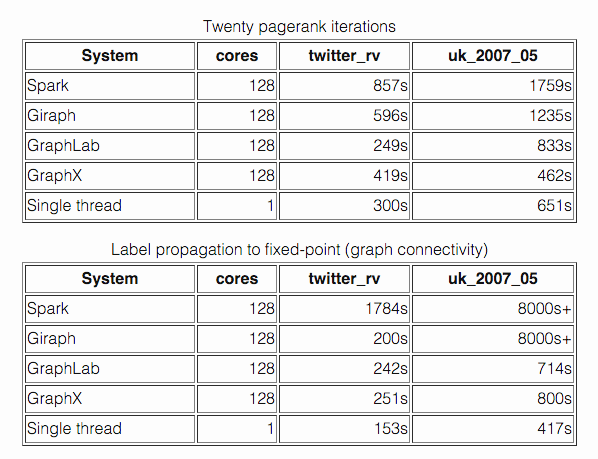
\includegraphics[width=0.80\textwidth]{images/pagerank.png}
\end{center}


\end{frame}



\begin{frame}
\frametitle{Takeaways}


\begin{changemargin}{1cm}

\begin{itemize}
\item    ``If you are going to use a big data system for yourself, see if it is faster than your laptop.''\\[1em]
\item    ``If you are going to build a big data system for others, see that it is faster than my laptop.''
\end{itemize}

\end{changemargin}
\end{frame}




\begin{frame}
\frametitle{Movie Hour, featuring NoSQL Bane}

Let's take a humorous look at cloud computing: James Mickens' session from Monitorama PDX 2014. 

\begin{center}
	
\includegraphics[width=0.5\textwidth]{images/bane.jpg}
\end{center}

\begin{center}
\url{https://vimeo.com/95066828}
\end{center}


\end{frame}

\end{document}

